\documentclass{article}\usepackage[]{graphicx}\usepackage[]{color}
%% maxwidth is the original width if it is less than linewidth
%% otherwise use linewidth (to make sure the graphics do not exceed the margin)
\makeatletter
\def\maxwidth{ %
  \ifdim\Gin@nat@width>\linewidth
    \linewidth
  \else
    \Gin@nat@width
  \fi
}
\makeatother

\definecolor{fgcolor}{rgb}{0.345, 0.345, 0.345}
\newcommand{\hlnum}[1]{\textcolor[rgb]{0.686,0.059,0.569}{#1}}%
\newcommand{\hlstr}[1]{\textcolor[rgb]{0.192,0.494,0.8}{#1}}%
\newcommand{\hlcom}[1]{\textcolor[rgb]{0.678,0.584,0.686}{\textit{#1}}}%
\newcommand{\hlopt}[1]{\textcolor[rgb]{0,0,0}{#1}}%
\newcommand{\hlstd}[1]{\textcolor[rgb]{0.345,0.345,0.345}{#1}}%
\newcommand{\hlkwa}[1]{\textcolor[rgb]{0.161,0.373,0.58}{\textbf{#1}}}%
\newcommand{\hlkwb}[1]{\textcolor[rgb]{0.69,0.353,0.396}{#1}}%
\newcommand{\hlkwc}[1]{\textcolor[rgb]{0.333,0.667,0.333}{#1}}%
\newcommand{\hlkwd}[1]{\textcolor[rgb]{0.737,0.353,0.396}{\textbf{#1}}}%

\usepackage{framed}
\makeatletter
\newenvironment{kframe}{%
 \def\at@end@of@kframe{}%
 \ifinner\ifhmode%
  \def\at@end@of@kframe{\end{minipage}}%
  \begin{minipage}{\columnwidth}%
 \fi\fi%
 \def\FrameCommand##1{\hskip\@totalleftmargin \hskip-\fboxsep
 \colorbox{shadecolor}{##1}\hskip-\fboxsep
     % There is no \\@totalrightmargin, so:
     \hskip-\linewidth \hskip-\@totalleftmargin \hskip\columnwidth}%
 \MakeFramed {\advance\hsize-\width
   \@totalleftmargin\z@ \linewidth\hsize
   \@setminipage}}%
 {\par\unskip\endMakeFramed%
 \at@end@of@kframe}
\makeatother

\definecolor{shadecolor}{rgb}{.97, .97, .97}
\definecolor{messagecolor}{rgb}{0, 0, 0}
\definecolor{warningcolor}{rgb}{1, 0, 1}
\definecolor{errorcolor}{rgb}{1, 0, 0}
\newenvironment{knitrout}{}{} % an empty environment to be redefined in TeX

\usepackage{alltt}
\usepackage{amsmath}
\DeclareMathOperator*{\argmin}{arg\,min}
\def\betahat{{\widehat\beta}}
\IfFileExists{upquote.sty}{\usepackage{upquote}}{}
\begin{document}



\section{Notation}

Let $C$ be a set of observed covariates, $A$ be an indicator of treatment, and $Y_a$ be the outcome observed under $A=a$. The observed outcome is given by $Y = AY_1 + (1-A)Y_0$. 

We are interested in comparing features of the marginal distributions of the potential outcomes. Let $f_{Y_a}$ denote the marginal distribution of potential outcome $Y_a$ (with CDF given by $F_{Y_a}$). We are interested in features of these distributions, which we will either describe through the quantiles or the mean. 

\begin{align*}
  E(Y_a) &= \int y f_{Y_a}(y) \partial y \\
  Q_{Y_a}(\tau) &= F^{-1}_{Y_a}(\tau)
\end{align*}

Examples of comparisons are the average causal effect (ATE), $E(Y_1-Y_0)$, the median causal effect, $Q_{Y_1}(0.5)-Q_{Y_0}(0.5)$, and more generally, the $p^{th}$ quantile causal effect, $Q_{Y_1}(p)-Q_{Y_0}(p)$.

A few notes. First, the expected value is the integral of the quantile function:

\begin{align*}
  E(Y_a) &= \int_0^1 Q_{Y_a}(p) \partial p
\end{align*}

\noindent Second, if we view the quantile causal effect as a function, then we can consider estimating the quantile effect for all $p$:

\begin{align*}
  QE(p) &= Q_{Y_1}(p)-Q_{Y_0}(p)
\end{align*}

\noindent Finally, combining the first two notes, we get:

\begin{align*}
  ATE &= E(Y_1-Y_0) = \int_0^1 QE(p) \partial p
\end{align*}

\section{Main assumptions}

The primary assumption will be strong ignorability, 

\begin{align*}
  (Y_1,Y_0) \bot A | C
\end{align*}

\noindent Based on Rubin, we know that this implies 

\begin{align*}
  (Y_1,Y_0) \bot A | e(C)
\end{align*}

\noindent where $e(C)=P(A=1|C)$ is known as the propensity score. The implication of strong ignorability is that the potential outcomes are independent of the treatment assignment conditional on the propensity score. That is, conditional on the propensity score, we can ignore the treatment assignment mechanism when describing features of the potential outcomes. In most applications of causal inference, we focus on the ATE. However, strong ignorability makes a statement about the entire distribution of the potential outcomes, so that we can make comparisons between any feature of the potential outcomes of interest (e.g. quantiles). 

There is stuff out there about local ignorability, or something like that. I've seen it in the context of regression discontinuity designs. Probably should have a look. 

We will also need SUTVA. No big deal. 

\section{Local quantile regression}

We will use local quantile regression to estimate $QE(p)$ around a given value of the propensity score. In other words, we will estimate the conditional quantile effect $QE(p|e(C)=\psi)$ using local quantile regression, where locality is based on the propensity score.

For a given value of the propensity score $\psi$, we seek to minimize

\begin{align*}
  \sum_i w_i \rho_\tau( Y_i - f(X_i))
\end{align*}

where $w_i$ is a weight and $\rho_\tau(u)=u(\tau-I(u<0))$. We choose the weight based on a kernel function, $K(.)$, and the bandwidth, $h$. Specifically, $w_i=K( \frac{\psi-e(C_i)}{h})$. Since the kernel function weights more heavily the observations that have propensity score close to $\psi$, we are estimating a local (in the PS) quantile effect. I'm sure we could somehow modify strong ignorability to explicity take into account the localness of the procedure. 

So we have the $\tau^{th}$ quantile effect around $e(C)=\psi$

\begin{align*}
  \betahat_\tau(\psi) = \widehat{QE}(p|e(C)=\psi) = \argmin_\beta \sum_i K\left( \frac{\psi-e(C_i)}{h}\right) \rho_\tau( Y_i - \beta_0 - \beta_1 A_i)
\end{align*}

\subsection{Estimating conditional ATE}

Let the conditional ATE be given by $ \beta(\psi) = E(Y_1-Y_0|e(C)=\psi)$. Using relationship between the quantiles and mean above, we can estimate the conditional ATE as:

\begin{align*}
   \betahat(\psi) &= \int_0^1 \betahat_\tau(\psi) \partial \tau
\end{align*}

\subsection{Estimating marginal quantile effects}

Let the marginal quantile be given by $ \beta_\tau = \int_0^1 QE(p|e(C)=\psi) f_{e(C)}(\psi) \partial \psi$. Note that our implementation creates a grid over the PS....so the integral will be a sum over our grid points:

\begin{align*}
   \betahat_\tau &=  \int_0^1 \betahat_\tau(\psi) \widehat{f}_{e(C)}(\psi) \partial \psi \\
   \widehat{f}_{e(C)}(x) &= \frac{1}{nh} \sum_{i=1}^n K\left( \frac{x-e(C_i)}{h}\right)
\end{align*}



\section{R code example}

First, we fit the model and suppress all output. So we don't see anything here!



Next, we run the code to produce the heatmaps!
\begin{knitrout}
\definecolor{shadecolor}{rgb}{0.969, 0.969, 0.969}\color{fgcolor}\begin{kframe}
\begin{alltt}
\hlkwd{heatmap.localQ}\hlstd{(}\hlkwc{fit}\hlstd{=out ,} \hlkwc{Ytype}\hlstd{=}\hlstr{"quantile"} \hlstd{,} \hlkwc{pch}\hlstd{=}\hlnum{16} \hlstd{,} \hlkwc{xlab}\hlstd{=}\hlstr{"PS"}\hlstd{)}
\end{alltt}
\end{kframe}

{\centering 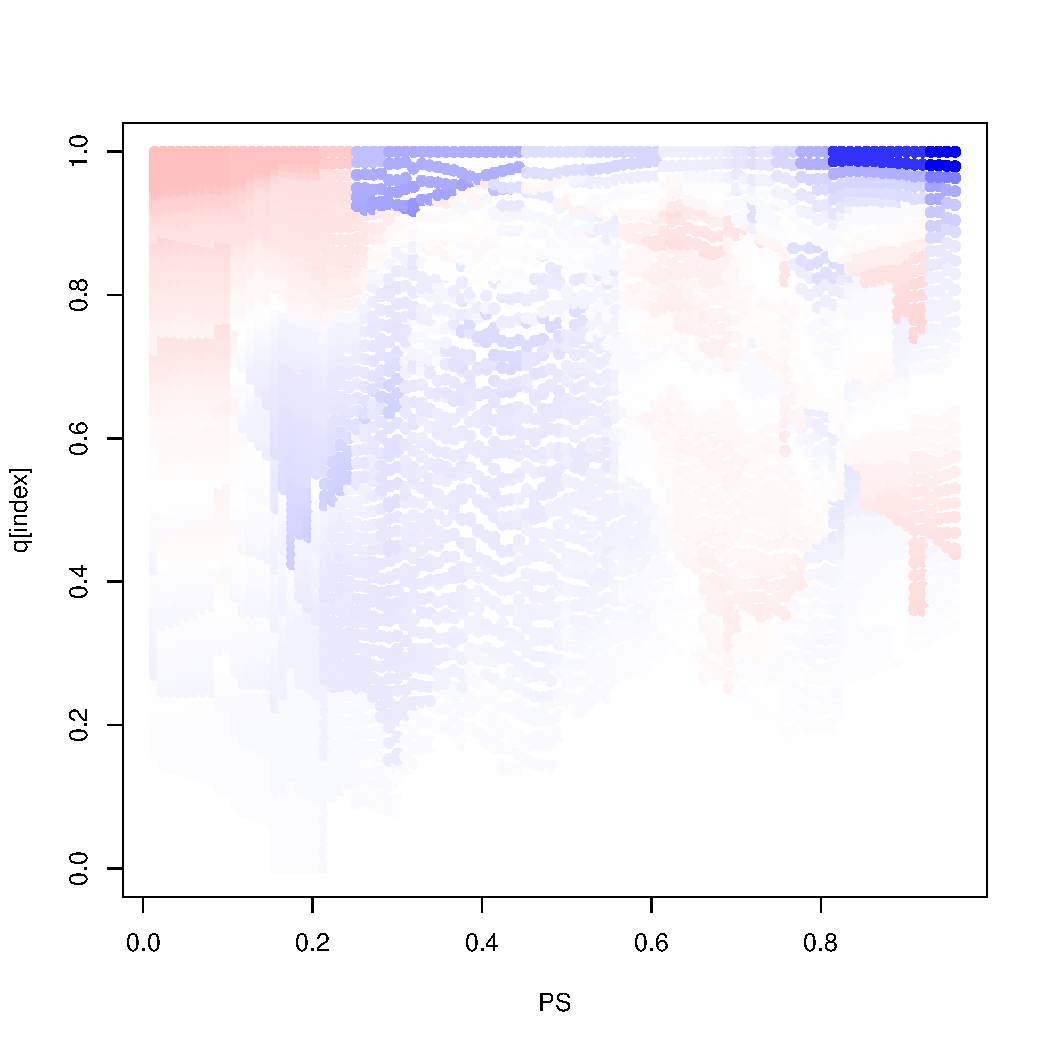
\includegraphics[width=\maxwidth]{figures/lalonde-heatmap-1} 

}



\end{knitrout}

Next, we run the code to produce the mean plot!
\begin{knitrout}
\definecolor{shadecolor}{rgb}{0.969, 0.969, 0.969}\color{fgcolor}\begin{kframe}
\begin{alltt}
\hlkwd{plot.Qmean}\hlstd{(}\hlkwc{fit}\hlstd{=out ,} \hlkwc{add}\hlstd{=F ,} \hlkwc{col}\hlstd{=}\hlstr{'blue'} \hlstd{,} \hlkwc{xlab}\hlstd{=}\hlstr{"PS"} \hlstd{,} \hlkwc{ylab}\hlstd{=}\hlstr{"Effect"}\hlstd{)}
\end{alltt}
\end{kframe}

{\centering 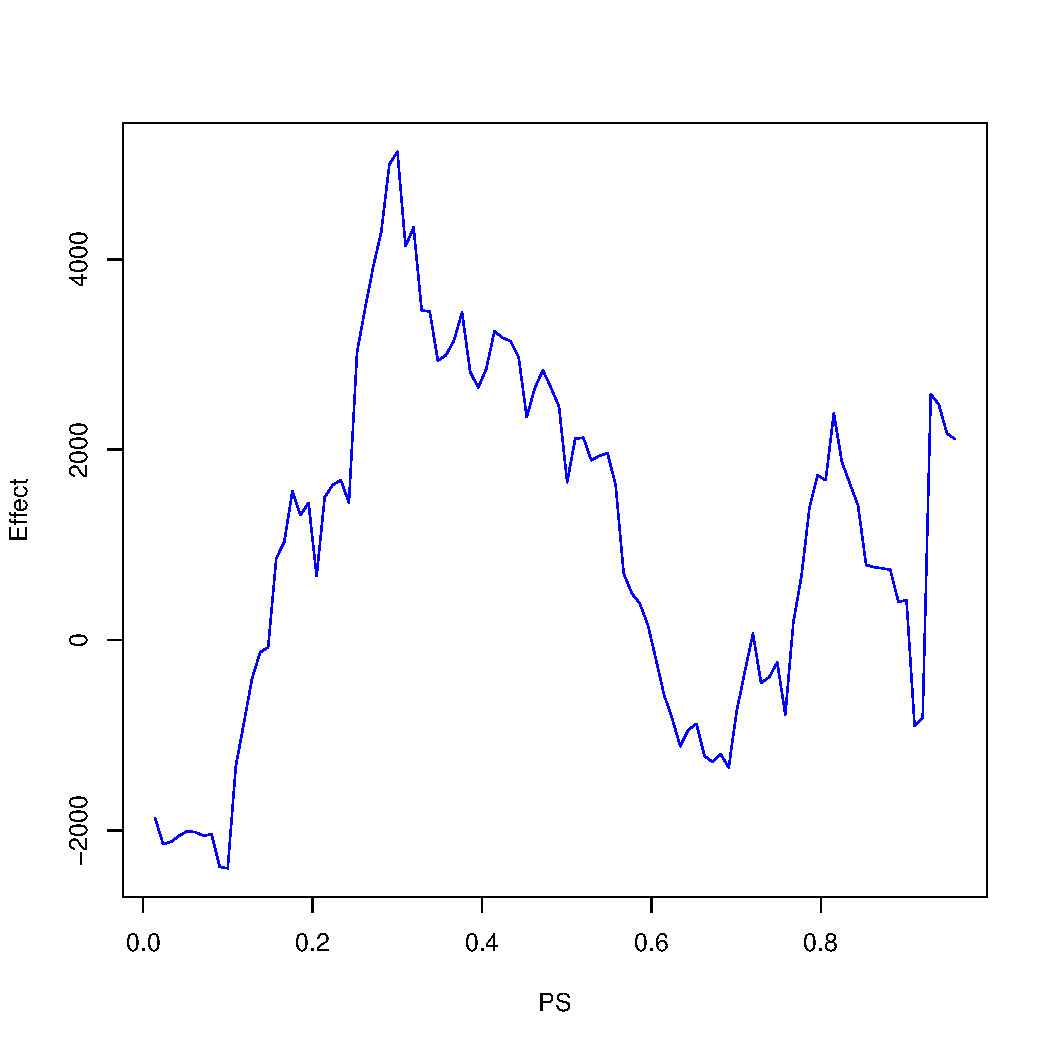
\includegraphics[width=\maxwidth]{figures/lalonde-meanplot-1} 

}



\end{knitrout}

Next, we run the code to produce the quantile plot!
\begin{knitrout}
\definecolor{shadecolor}{rgb}{0.969, 0.969, 0.969}\color{fgcolor}\begin{kframe}
\begin{alltt}
\hlkwd{plot.Qavg}\hlstd{(}\hlkwc{fit}\hlstd{=out ,} \hlkwc{Ytype}\hlstd{=}\hlstr{"quantile"} \hlstd{,} \hlkwc{type}\hlstd{=}\hlstr{'l'} \hlstd{,} \hlkwc{col}\hlstd{=}\hlstr{'blue'} \hlstd{,} \hlkwc{xlab}\hlstd{=}\hlstr{"quantile of Y(0)"} \hlstd{,} \hlkwc{ylab}\hlstd{=}\hlstr{"Effect"}\hlstd{)}
\end{alltt}
\end{kframe}

{\centering 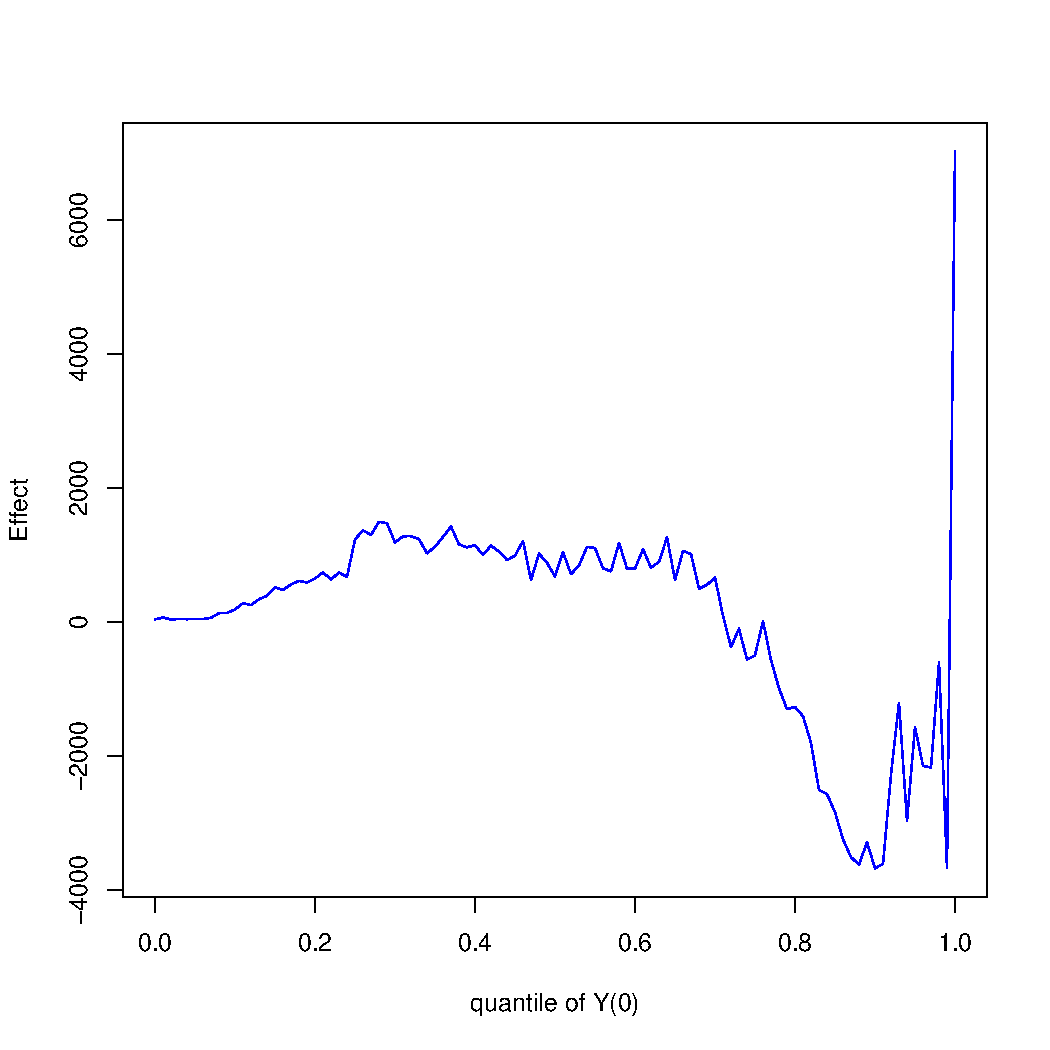
\includegraphics[width=\maxwidth]{figures/lalonde-Qplot-1} 

}



\end{knitrout}


\section{Substance abuse example from Beth Ann}



\subsection{SFS}
\begin{knitrout}
\definecolor{shadecolor}{rgb}{0.969, 0.969, 0.969}\color{fgcolor}\begin{kframe}
\begin{alltt}
\hlkwd{heatmap.localQ}\hlstd{(}\hlkwc{fit}\hlstd{=out.sfs ,} \hlkwc{Ytype}\hlstd{=}\hlstr{"quantile"} \hlstd{,} \hlkwc{pch}\hlstd{=}\hlnum{16} \hlstd{,} \hlkwc{xlab}\hlstd{=}\hlstr{"PS"}\hlstd{)}
\end{alltt}
\end{kframe}

{\centering 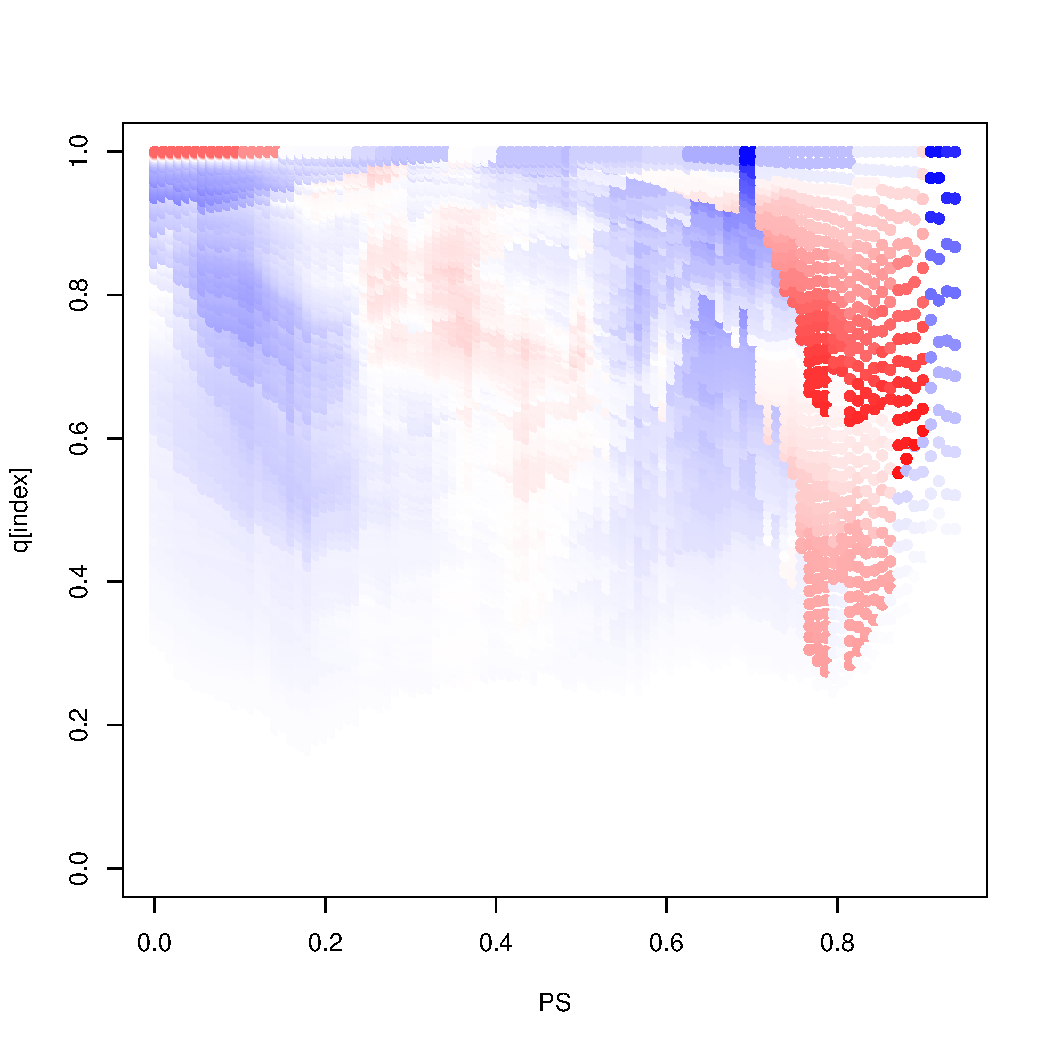
\includegraphics[width=\maxwidth]{figures/SFS-heatmap-1} 

}



\end{knitrout}
\subsection{SPS}
\begin{knitrout}
\definecolor{shadecolor}{rgb}{0.969, 0.969, 0.969}\color{fgcolor}\begin{kframe}
\begin{alltt}
\hlkwd{heatmap.localQ}\hlstd{(}\hlkwc{fit}\hlstd{=out.sps ,} \hlkwc{Ytype}\hlstd{=}\hlstr{"quantile"} \hlstd{,} \hlkwc{pch}\hlstd{=}\hlnum{16} \hlstd{,} \hlkwc{xlab}\hlstd{=}\hlstr{"PS"}\hlstd{)}
\end{alltt}
\end{kframe}

{\centering 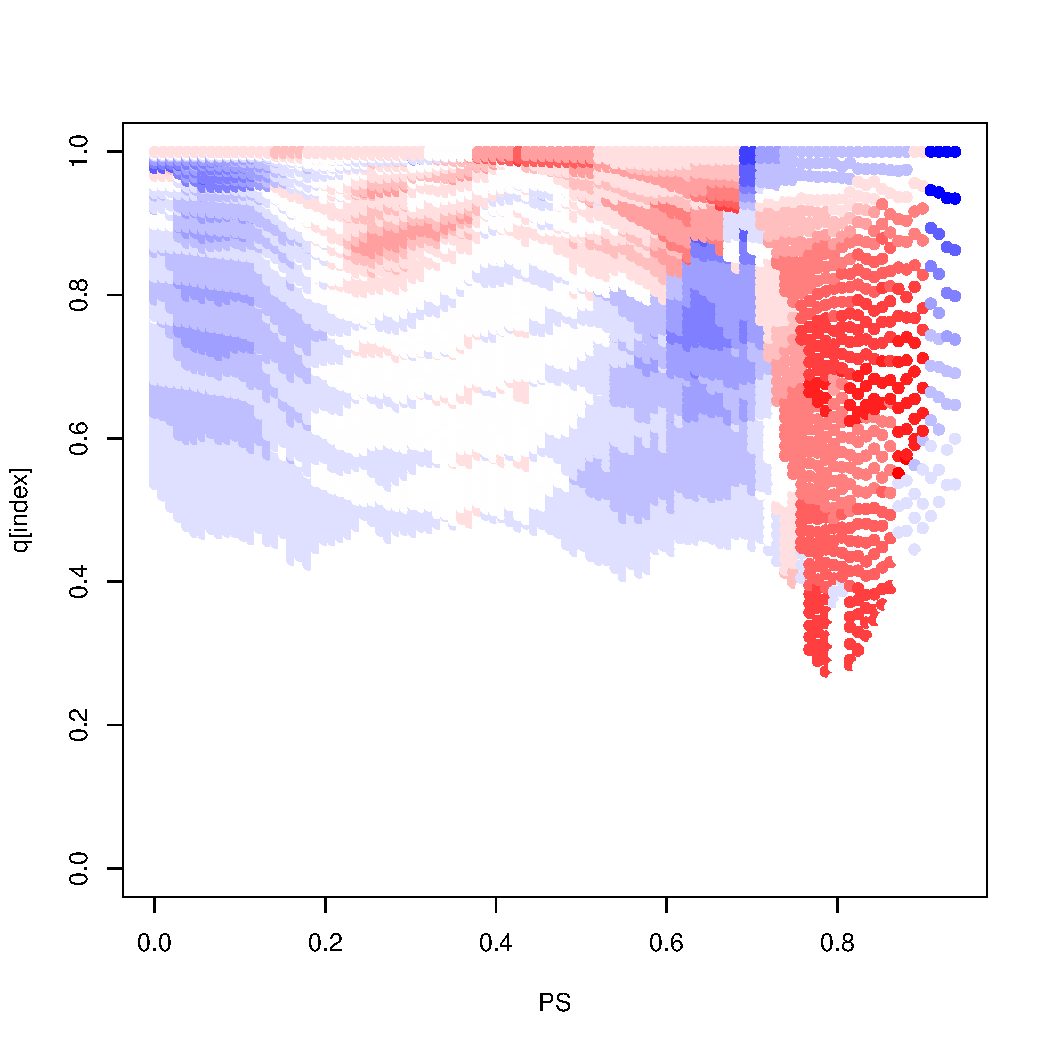
\includegraphics[width=\maxwidth]{figures/SPS-heatmap-1} 

}



\end{knitrout}
\subsection{EPS}
\begin{knitrout}
\definecolor{shadecolor}{rgb}{0.969, 0.969, 0.969}\color{fgcolor}\begin{kframe}
\begin{alltt}
\hlkwd{heatmap.localQ}\hlstd{(}\hlkwc{fit}\hlstd{=out.eps ,} \hlkwc{Ytype}\hlstd{=}\hlstr{"quantile"} \hlstd{,} \hlkwc{pch}\hlstd{=}\hlnum{16} \hlstd{,} \hlkwc{xlab}\hlstd{=}\hlstr{"PS"}\hlstd{)}
\end{alltt}
\end{kframe}

{\centering 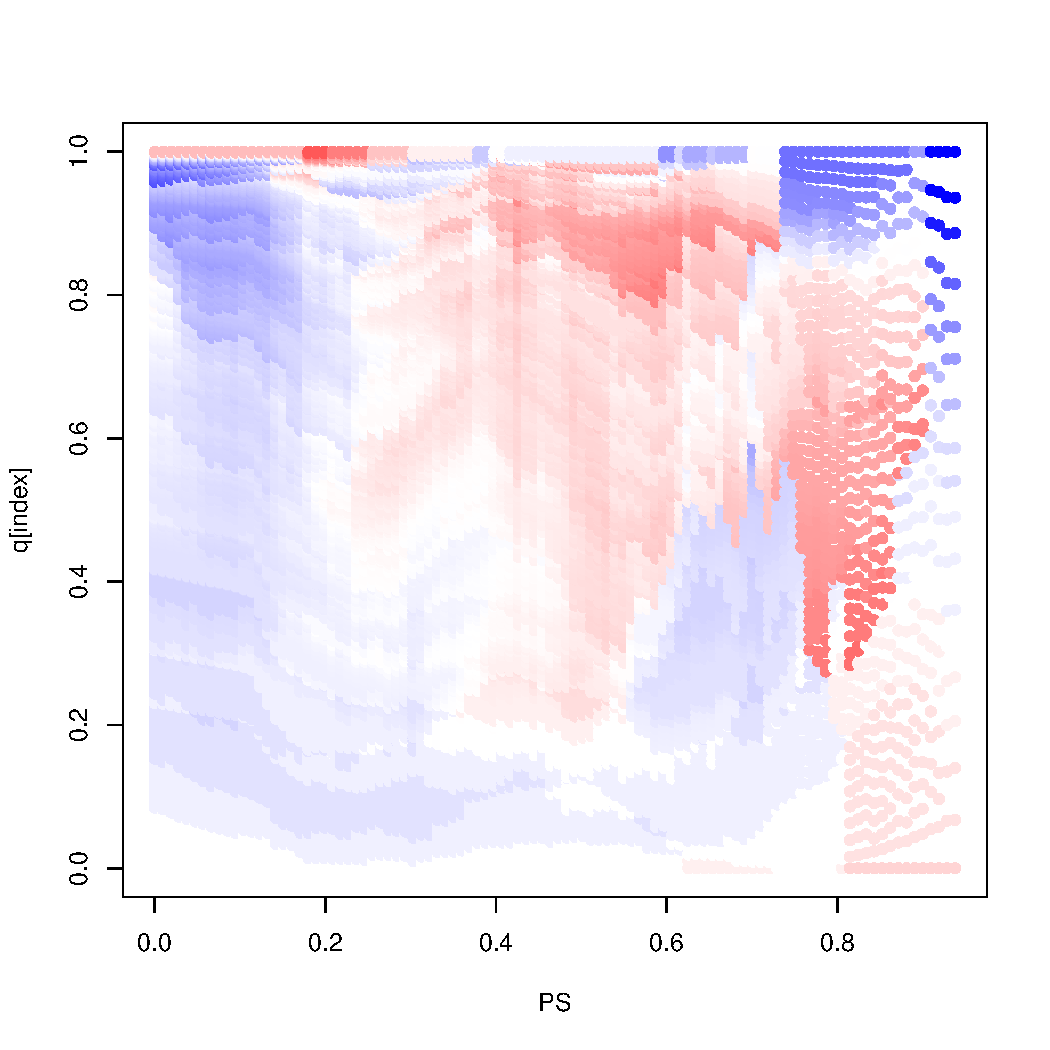
\includegraphics[width=\maxwidth]{figures/EPS-heatmap-1} 

}



\end{knitrout}
\subsection{SDS}
\begin{knitrout}
\definecolor{shadecolor}{rgb}{0.969, 0.969, 0.969}\color{fgcolor}\begin{kframe}
\begin{alltt}
\hlkwd{heatmap.localQ}\hlstd{(}\hlkwc{fit}\hlstd{=out.sds ,} \hlkwc{Ytype}\hlstd{=}\hlstr{"quantile"} \hlstd{,} \hlkwc{pch}\hlstd{=}\hlnum{16} \hlstd{,} \hlkwc{xlab}\hlstd{=}\hlstr{"PS"}\hlstd{)}
\end{alltt}
\end{kframe}

{\centering 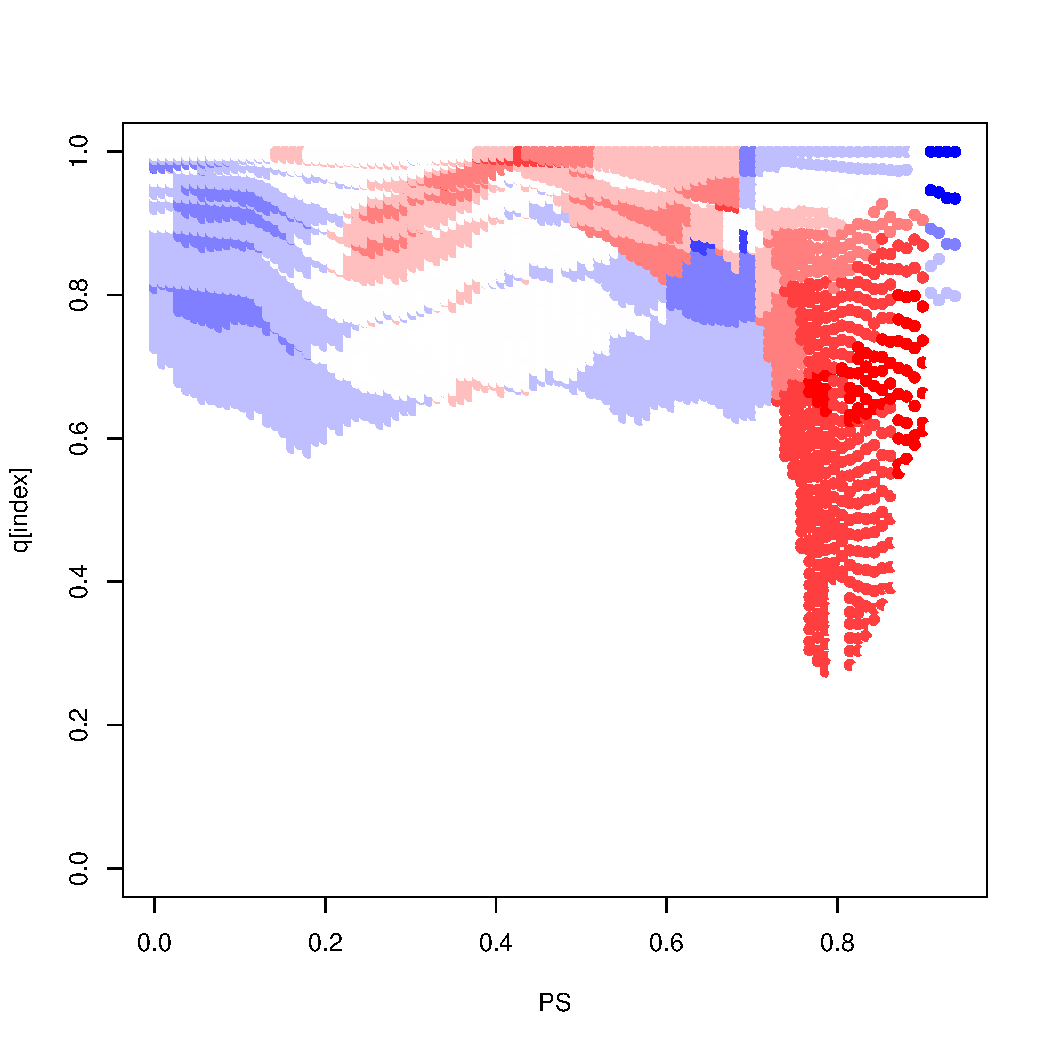
\includegraphics[width=\maxwidth]{figures/SDS-heatmap-1} 

}



\end{knitrout}

\end{document}


